\chapter{Open heavy-flavour production in pp collisions}

\lettrine[lines=6,findent=0.pt]{O}{pen heavy-flavour} hadrons, made of a heavy quark (charm or beauty) along with lighter quarks, are exclusively formed in high-momentum transfer processes due to their large mass of approximately 1.27 \gevcc and 4.18 \gevcc for charm and beauty quarks, respectively. As such, they are created in the early stages of the collision, and their production cross-section in the partonic interaction can be evaluated perturbatively using QCD. Studying the production of open heavy-flavour hadrons in proton-proton collisions not only provides a crucial test of the perturbative QCD framework, but also allows to set constraints on models. Furthermore, such measurements in proton-proton collisions, where the production of a deconfined medium is not expected due to the low energy densities reached, are necessary ingredients for the study of heavy-ion collisions, where the properties of the QGP can be investigated. 

\section{Factorisation theorems}
The production of open heavy-flavour hadrons in proton-proton collisions can be described using the factorisation theorems~\cite{Collins:1989gx}, which allow for the separation of short-distance, perturbative behaviour from the long-distance, non-perturbative phenomena. The total production cross-section can be expressed as
\begin{equation*}
    \sigma_{\text{pp}}^\mathrm{H} = \sum_\mathrm{a,b = g, q, \overline{q}} \int \de x_1 \de x_2 f_\mathrm{a/A}(x_1,\mu_F^2) f_\mathrm{b/B}(x_2,\mu_F^2) \hat{\sigma}_\mathrm{ab \rightarrow c} (x_1,x_2,\mu_F^2,\mu_R^2) D_\mathrm{c\rightarrow H}(z,\mu_F^2) \quad ,
\end{equation*}
i.e. the convolution of; i. the Parton Distribution Functions (PDFs) $f_\mathrm{a/A}(x_1,\mu_F^2)$ and $f_\mathrm{b/B}(x_2,\mu_F^2)$, describing the probability of finding a parton a in the proton A carrying a fraction $x_1$ of the proton's momentum, and a parton b in the proton B carrying a fraction $x_2$ of its momentum, respectively; ii. the hard partonic scattering cross-section $\hat{\sigma}_\mathrm{ab \rightarrow c} (x_1,x_2,\mu_F^2,\mu_R^2)$, defining the probability of producing the final state c from the collision of partons a and b; and iii. the Fragmentation Functions (FFs) $D_\mathrm{c\rightarrow H}(z,\mu_F^2)$, which describe the probability of a parton of type c fragmenting into a heavy-flavour hadron H with a momentum fraction $z$. While the PDFs and FFs are non-perturbative quantities, determined from experimental data and then regarded as universal across different processes, the hard partonic scattering cross-section can be perturbatively calculated using QCD, albeit requiring specific evaluations for each process. Factorisation theorems have been widely used to describe the production of open heavy-flavour hadrons in proton-proton collisions, and have proven to be successful in modeling experimental data. Figure~\ref{fig:ppDmeson} shows the production cross-section of prompt and non-prompt $\mathrm{D^0}$-mesons in proton-proton collisions at $\sqrt{s} = 13$ TeV measured at midrapidity ($\lvert y\rvert<0.5$) as a function of the transverse momentum by the ALICE experiment~\cite{ALICE:2021mgk}, and compared to FONLL calculations~\cite{Cacciari:1998it}. The term \emph{prompt} refers to charm-hadrons directly produced in the hadronisation of a charm quark or through the strong decay of a directly produced excited charm-hadron state, while \emph{feed-down} charm-hadrons are produced in the decay of a hadron containing a beauty quark. The FONLL predictions are in good agreement with the non-prompt $\mathrm{D^0}$-meson production cross-section, whereas the prompt contribution lies at the upper edge of the theoretical uncertainty band, albeit being described within the uncertainties.  Similar trends are observed in the production of other open heavy-flavour hadrons across different experimental facilities, such as the Tevatron, RHIC and LHC.

\begin{figure}[htb]
    \centering
    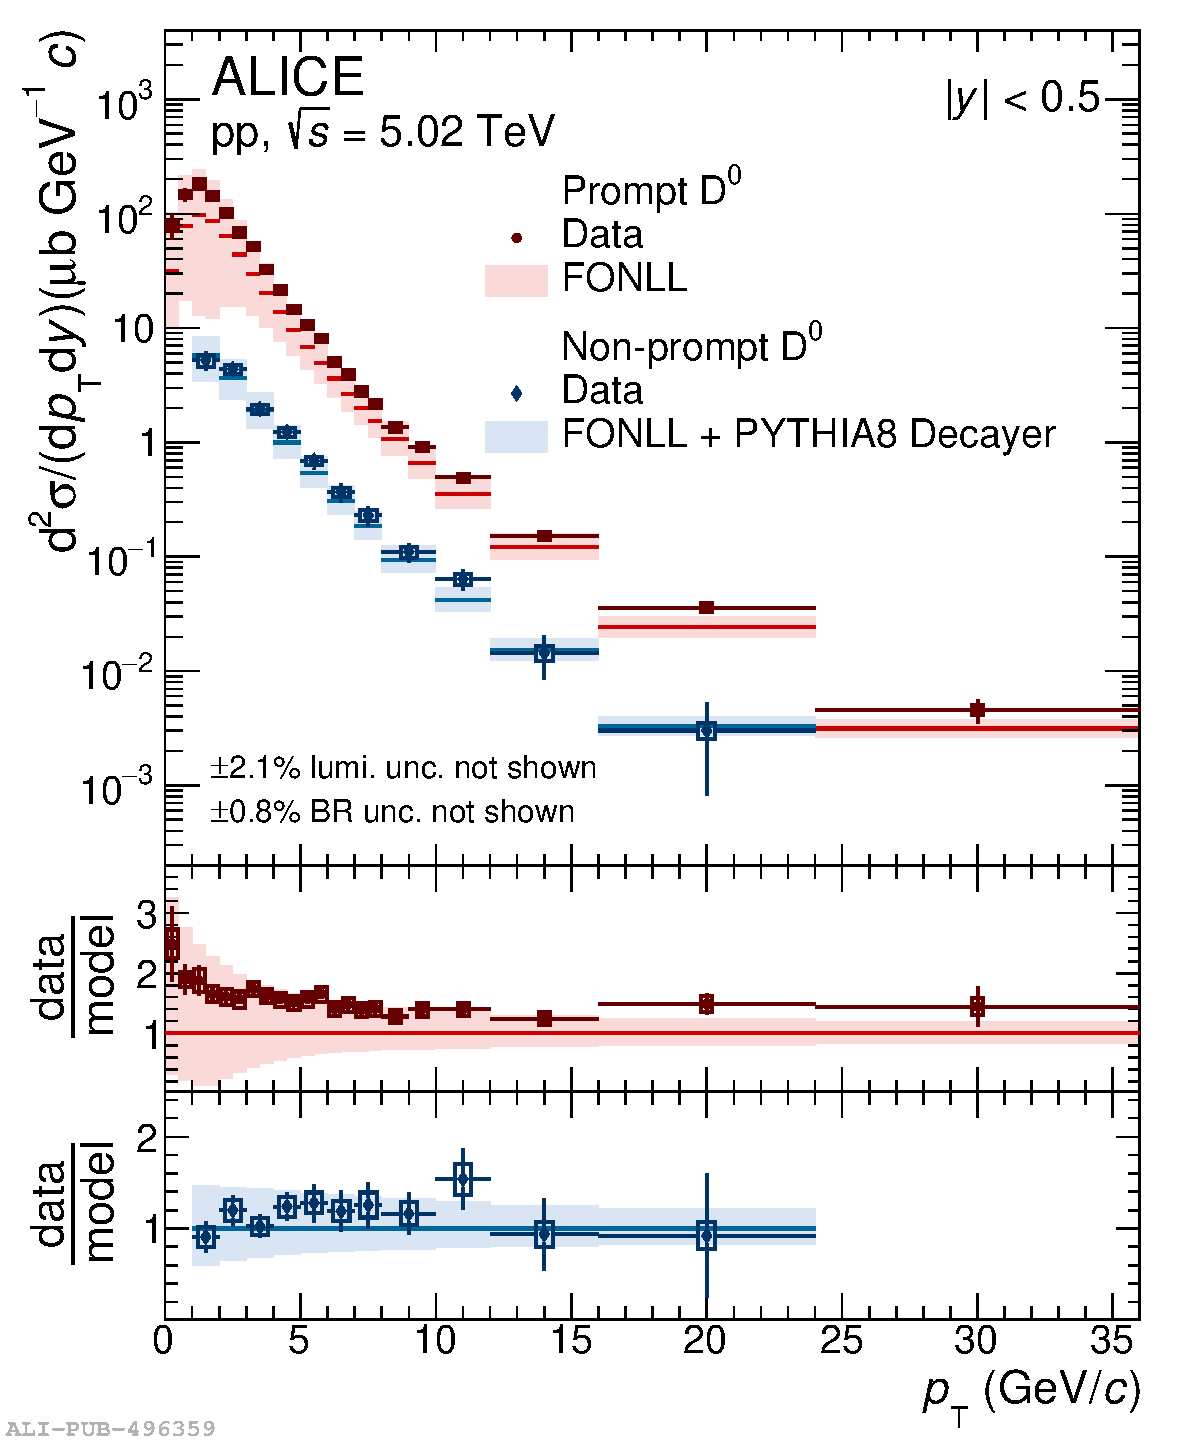
\includegraphics[width=0.6\linewidth]{Figures/Chapter 2/CrossSectionD0_Prompt_NonPrompt_pp5TeV_vsFONLL_Pythia8_BRnative_1.pdf}
    \caption{\pt-differential production cross-section of prompt and non-prompt $\mathrm{D^0}$-mesons~\cite{ALICE:2021mgk} compared to predictions obtained with FONLL calculations~\cite{Cacciari:1998it} combined with PYTHIA~8~\cite{Sjostrand:2014zea} for the $\mathrm{H_b \rightarrow D^0+X}$ decay kinematics.}
    \label{fig:ppDmeson}
\end{figure}

\subsection{Parton Distribution Functions}
\subsubsection{Deep inelastic scattering}
The PDFs are non-perturbative quantities describing the probability of finding a parton carrying a fraction $x$ of the proton's momentum in the initial state of a process. The first experimental evidence revealing the partonic structure of the proton emerged from deep inelastic scattering experiment carried out at the Stanford Linear Accelerator Center (SLAC) in the 1960s~\cite{Friedman:1972sy}, where an electron was scattered off a proton, and the transeferred momentum $q$ was measured. The cross-section for deep inelastic scattering can be defined in terms of the Lorentz invariant variables $Q^2 = -q^2$ and $x = \frac{Q^2}{2P\cdot q}$, yielding
\begin{equation*}
    \frac{\de^2\sigma}{\de x \de Q^2} = \frac{4\pi\alpha^2}{xQ^4} \left[ \left(1-y\right)F_2(x,Q^2) - xy^2F_1(x,Q^2) \right]\quad ,
\end{equation*}
where $y=Q^2/(sx)$, $s = (P+p_\mathrm{e})^2$ denotes the centre-of-mass energy of the electron-proton system, and the structure functions $F_1(x,Q^2)$ and $F_2(x,Q^2)$ represent an extension of the form factors for elastic scattering.
The first measurements of high-energy inclusive inelastic scattering experiments were performed using a 20~GeV linear accelerator at SLAC, and showed that the structure functions $F_1(x,Q^2)$ and $F_2(x,Q^2)$ were independent of $Q^2$ at fixed $x$ within the studied $1<~Q^2~<~10$~\gevcc range. This was in contrast with the behavior observed for the proton elastic form factors, where a decrease of two orders of magnitude was observed within the same $Q^2$ interval. The observed behaviour was predicted by Bjorken in 1968 for $Q^2 \rightarrow \infty$~\cite{Bjorken:1968dy}, and is known as \emph{Bjorken scaling}. A physical interpretation of the phenomena arrived just one year later, in 1969, with Feynman's parton model~\cite{Feynman:1969ej}, which described the interaction in terms of elastic scattering of the probe off a point-like constituent (parton) within the proton. This model explains the scale-invariance property of the proton structure functions, as the scattering centres are assumed structure-less. In this picture, the Bjorken variable $x$ acquires a new interpretation as the fraction of the proton momentum carried by the struck parton. The parton model also offers a straightforward definition of the structure functions in terms of the parton distribution functions $f_\mathrm{a}(x)$:
\begin{equation*}
    F_2(x,Q^2) = \sum_\mathrm{a} e_\mathrm{a}^2 x f_\mathrm{a}(x)\quad ,
\end{equation*}
where the sum is over partons with electric charge $e_\mathrm{a}$, and $f_\mathrm{a}$ are unknown, but universal functions for a given hadron, describing the probability of finding a parton of type a with a fraction $x$ of the proton's momentum. 

To explore the spin properties of the partons, the structure functions $F_1$ and $F_2$ were studied at different centre-of-mass energies. By investigating the relationship between the two structure functions, it was established that the partons have spin 1/2, as the Callan-Gross relation~\cite{Callan:1969uq}, which holds true for point-like Dirac particles, was found to be satisfied:
\begin{equation*}
    F_2(x,Q^2) = 2x F_1(x,Q^2)\quad .
\end{equation*}

In the next years, it became clear that additional constituents within the proton carry momentum but lack electric charge or weak charge, as the so-called momentum sum rule was not saturated by the measured PDFs in electron and neutrino scatterings. This missing momentum was attributed to gluons, which were discovered in the 1970s and are the field quanta of the strong force.

\subsubsection{Bjorken scaling violation}
\begin{figure}[htb]
    \centering
    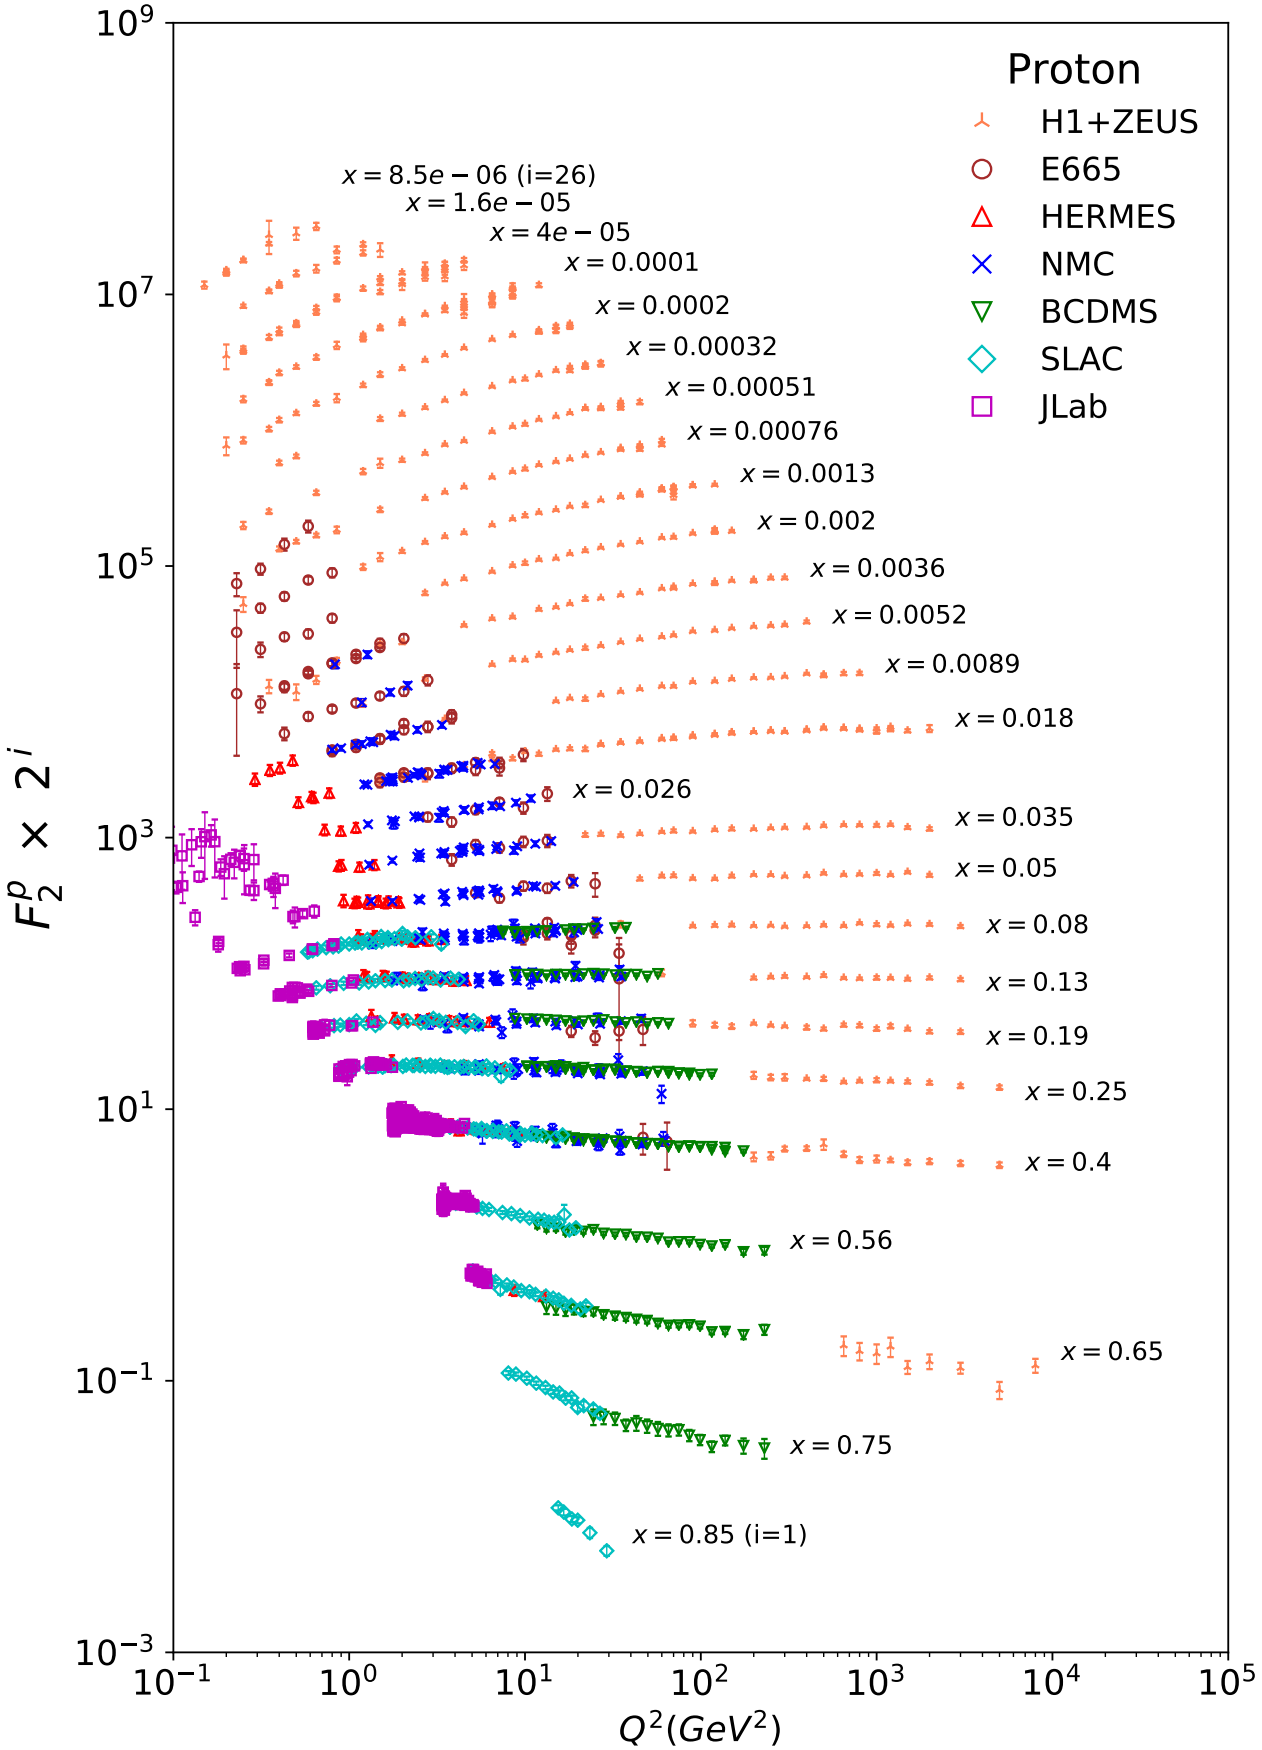
\includegraphics[width=0.6\linewidth]{Figures/Chapter 2/F2Results.png}
    \caption{The proton structure function $F^p_2$ measured in electromagnetic scattering of electrons and positrons on protons, and for electrons/positrons and muons on a fixed target~\cite{pdg}.}
    \label{fig:scaling_violation}
\end{figure}
By the late 1970s, measurements of the structure functions at larger $Q^2$ values taken at CERN and Desy revealed that the Bjorken scaling was violated, i.e. the structure functions were not $Q^2$ independent. Figure~\ref{fig:scaling_violation} shows measurements of the proton structure functions $F_2(x,Q^2)$ as a function of $Q^2$ for various values of $x$ taken from different experiments~\cite{pdg}. It is clear from the plot that structure functions present an increasing trend as a function of $Q^2$ at low $x$, and a decreasing trend as a function of $Q^2$ at high $x$. 

The parton model fails to explain this behaviour, as it relies on the assumption that the transferred energy is sufficiently large to neglect the the proton and its constituents' masses, as well as the interactions among partons. In particular, the partons' transverse momentum with respect to the proton momentum is neglected. The key point in understanding the Bjorken scaling violation comes from QCD and is that the parton's transverse momentum is not in fact restricted to be small. A quark, for instance, can emit a gluon and acquire large transverse momentum $k_T$ with a probability proportional to $\als \de k_T/k_T^2$ at large $k_T$. The integral extends up to the kinematic limit $k_T\sim Q^2$, giving rise to contributions proportional to $\als\mathrm{log}Q^2$, which break scaling. The evolution of PDFs with $Q^2$ from a parametrisation at a given $Q^2_0$ can be perturbatively described using the Dokshitzer-Gribov-Lipatov-Altarelli-Parisi (DGLAP) evolution equations~\cite{Gribov:1972ri,Dokshitzer:1977sg,Altarelli:1977zs}, which requires the introduction of a new arbitrary scale, at which the factorisation of the non-perturbative processes happens: the factorisation scale $\mu_F$. There exists a wide range of PDFs parametrisations, such as the NNPDF~\cite{NNPDF:2021njg}, CTEQ~\cite{Dulat:2015mca} and MMHT~\cite{Harland-Lang:2014zoa}, which are determined from global fits to a wide range of experimental data, such as deep inelastic scattering, Drell-Yan, and jet production.

\subsection{Partonic cross-section}
\begin{figure}[htb]
    \centering
    \begin{tikzpicture}
      \begin{feynman}
        \vertex (a);
        \vertex [above=1cm of a] (b) {q};
        \vertex[below=1cm of a] (c) {$\overline{\mathrm{q}}$};
        \vertex[right=1cm of a] (d);
        \vertex[right=0.7cm of d] (e);
        \vertex[right=1.3cm of e] (f);
        \vertex[right=0.7cm of f] (g);
        \vertex[right=1cm of g] (h);
        \vertex[above=1cm of h] (i) {Q};
        \vertex[below=1cm of h] (j) {$\overline{\mathrm{Q}}$};
        \diagram* {
            (b) -- [fermion] (d) -- [fermion] (c),
            (d) -- [gluon] (e),
            (e) -- [gluon,  in=90, out=90, looseness=1.7] (f) -- [gluon,  in=-90, out=-90, looseness=1.7] (e),
            (f) -- [gluon] (g),
            (j) -- [fermion] (g) -- [fermion] (i),
        };
      \end{feynman}
    \end{tikzpicture}\quad
    \begin{tikzpicture}
        \begin{feynman}
          \vertex (a);
          \vertex [above=1cm of a] (b) {q};
          \vertex[below=1cm of a] (c) {$\overline{\mathrm{q}}$};
          \vertex[right=1cm of a] (d);
          \vertex[right=0.7cm of d] (e);
          \vertex[right=1.3cm of e] (f);
          \vertex[right=0.7cm of f] (g);
          \vertex[right=1cm of g] (h);
          \vertex[above=1cm of h] (i) {Q};
          \vertex[below=1cm of h] (j) {$\overline{\mathrm{Q}}$};
          \diagram* {
              (b) -- [fermion] (d) -- [fermion] (c),
              (d) -- [gluon] (e),
              (e) -- [fermion,  in=90, out=90, looseness=1.7] (f) -- [fermion,  in=-90, out=-90, looseness=1.7] (e),
              (f) -- [gluon] (g),
              (j) -- [fermion] (g) -- [fermion] (i),
          };
        \end{feynman}
      \end{tikzpicture}

    \vspace*{0.5cm}
    \begin{tikzpicture}
        \begin{feynman}
          \vertex (a);
          \vertex [above=1cm of a] (b) {q};
          \vertex[below=1cm of a] (c) {$\overline{\mathrm{q}}$};
          \vertex[right=1cm of a] (d);
          \vertex[right=1cm of d] (e);
          \vertex[right=1cm of e] (f);
          \vertex[above=1cm of f] (g) {Q};
          \vertex[below=1cm of f] (h) {$\overline{\mathrm{Q}}$};
          \vertex[right=0.5cm of e] (i);
          \vertex[below=0.5cm of i] (j);
          \diagram* {
              (b) -- [fermion] (d) -- [fermion] (c),
              (d) -- [gluon] (e),
              (h) -- [fermion] (e) -- [fermion] (g),
              (j) -- [gluon, edge label = g] (f),

          };
        \end{feynman}
      \end{tikzpicture}\quad
      \begin{tikzpicture}
        \begin{feynman}
            \vertex (a);
            \vertex [above=1cm of a] (b) {q};
            \vertex[below=1cm of a] (c) {$\overline{\mathrm{q}}$};
            \vertex[right=1cm of a] (d);
            \vertex[right=1cm of d] (e);
            \vertex[right=1cm of e] (f) ;
            \vertex[above=1cm of f] (g) {Q};
            \vertex[below=1cm of f] (h) {$\overline{\mathrm{Q}}$};
            \vertex[right=0.5cm of e] (i);
            \vertex[below=0.5cm of i] (j);
          \diagram* {
              (b) -- [gluon] (d) -- [gluon] (c),
              (d) -- [gluon] (e),
              (h) -- [fermion] (e) -- [fermion] (g),
              (j) -- [gluon, edge label = g] (f),

          };
        \end{feynman}
      \end{tikzpicture}\quad
      \begin{tikzpicture}
        \begin{feynman}
          \vertex (a) {g};
          \vertex[above=0.25cm of a] (spacing) {$ $  }; 
          \vertex[right=1.25cm of a] (b);
          \vertex[right=1.45cm of b] (c) {q};
          \vertex[below=1.75cm of a] (d) {q};
          \vertex[right=1.25cm of d] (e);
          \vertex[right=0.75cm of e] (f);
          \vertex[right=1cm of f] (g);
          \vertex[above=0.3cm of g] (h) {Q};
          \vertex[below=0.3cm of g] (j) {$\overline{\mathrm{Q}}$};
          \diagram* {
                (a) -- [gluon] (b),
                (d) -- [fermion] (e) -- [fermion] (b) -- [fermion] (c),
                (e) -- [gluon] (f),
                (j) -- [fermion] (f) -- [fermion] (h),
          };
        \end{feynman}
      \end{tikzpicture}\quad
    \caption{Feynman diagrams contributing to the first order corrections of the heavy-flavour production cross-section calculations.}
    \label{fig:NLO_diagrams}
\end{figure}


Because of their large masses, heavy quarks can only be produced through hard-scattering processes, characterized by momentum transfers of the order of $Q^2 \geq 4m^2_\mathrm{b,c}$. In this regime, the strong coupling constant is significantly smaller than unity, allowing for the perturbative calculation of the heavy quark production cross-section from partonic scattering using QCD. While predictions at next-to-next-to-next-to-leading order (N$^3$LO) are available for certain processes, such as Higgs production~\cite{Anastasiou:2015vya, Anastasiou:2016cez}, the current state-of-the-art calculations for heavy quark production are at next-to-leading order (NLO) with all-order resummation to next-to-leading logarithmic (NLL) accuracy in the limit where the \pt of a heavy quark is much larger than its mass~\cite{Cacciari:1998it}. The contributions arising at the NLO include 1-loop virtual corrections to the Born process and real emission of a gluon, and are reported in Fig~\ref{fig:NLO_diagrams}.

\subsection{Fragmentation Functions}
Quarks and gluons produced in hard-scattering processes will ultimately give rise to colourless observable hadrons. The associated process, known as hadronisation, is non-perturbative and is described by the Fragmentation Functions (FFs) $D_\mathrm{c\rightarrow H}(z,\mu_F^2)$, which describe the probability of a parton of type c fragmenting into a hadron H with a momentum fraction $z$. FFs are typically determined from experimental data, usually by analyzing the final-state hadrons produced in electron-positron collisions, where the initial momenta are well-known, and are then applied in the evaluation of cross-sections in other colliding systems, assuming that the relevant hadronisation processes are “universal”, i.e. independent of the collision energy and system. By studying the distribution of identified hadrons as a function of their momentum fraction z, it is possible to extract information about the fragmentation process. Similar to the PDFs, FFs also evolve with the energy scale of the interaction, and this evolution is described perturbatively by the DGLAP equations. 
\section{Modification of the hadronisation mechanism}
\begin{figure}[htb]
    \centering
    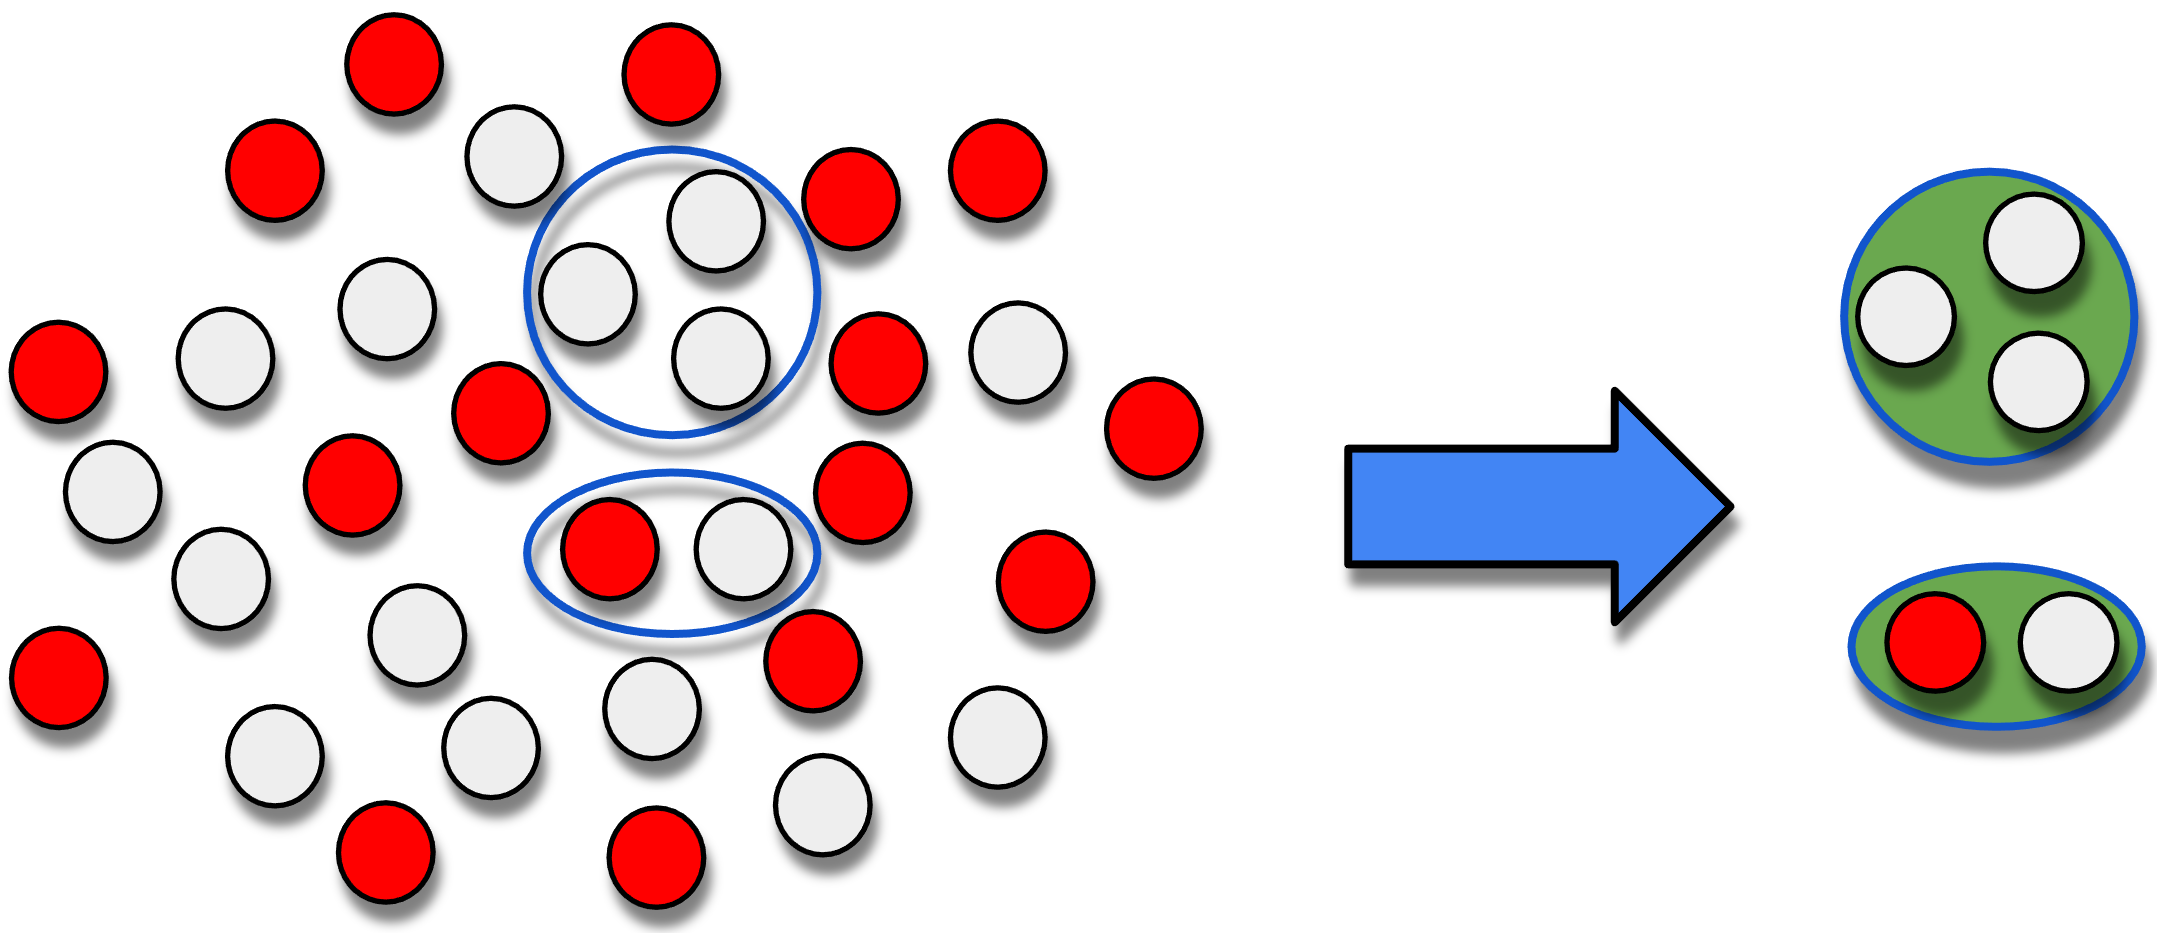
\includegraphics[width=0.7\linewidth]{Figures/Chapter 2/Coalescence.png}
    \caption{Representation of hadron production via recombination.}
\end{figure}

As outlined in Sec.~\ref{sec:high_pt}, the hadronisation process can be modified in the presence of a strongly-interacting deconfined medium. A novel mechanism for the production of hadrons, the recombination, can take place in the QGP. This process modifies the production of hadrons in heavy-ion collisions, so that the description of fragmentation functions derived from \ee collisions becomes inadequate. Only models implementing the coalescence mechanism can effectively describe the production of hadrons in these collisions. Intriguingly, models implementing recombination that successfully describe the production of hadrons in heavy-ion collisions, fail in doing so when this process is de-activated, as shown in Fig.~\ref{fig:D_recombination}. Recent measurements of charm-baryons production in proton-proton and proton-lead collisions~\cite{ALICE:2022exq,ALICE:xic0} have provided insightful results on the production of hadrons in such systems. Notably, models with hadronisation tuned on \ee collisions fail to describe the data, suggesting that coalescence could also play a role in small collision systems, and that the hadronisation process is not universal across different systems at all.

\begin{figure}[htb]
  \centering
  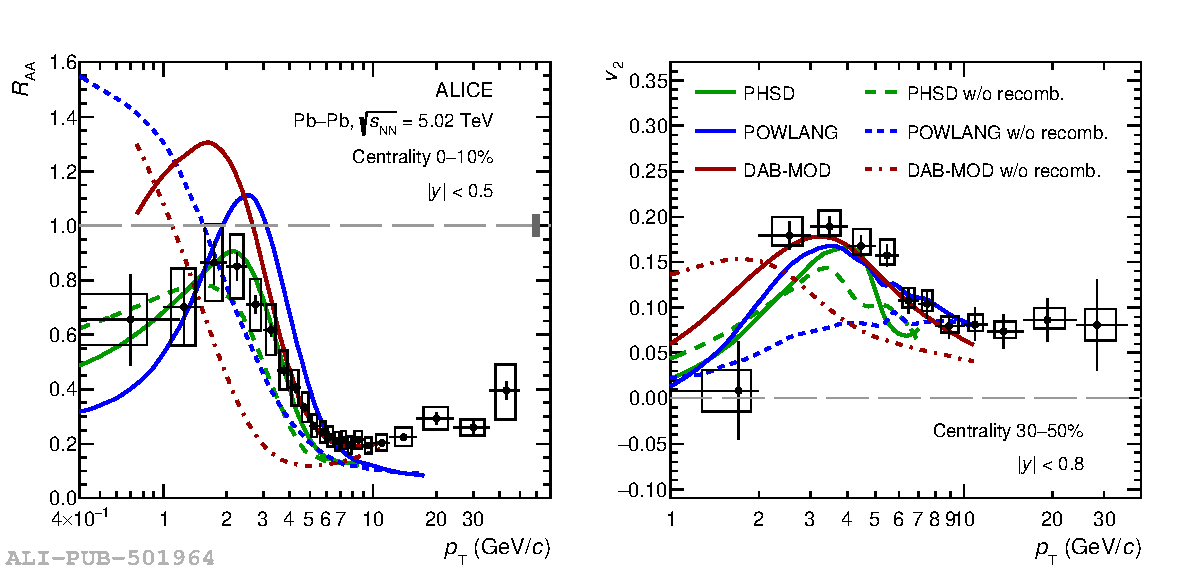
\includegraphics[width=\linewidth]{Figures/Chapter 2/D_Raa010_V23050_FragCoal_3models_1.pdf}
  \caption{Prompt D-meson $R_\mathrm{AA}$ in the 0--10\% centrality class (left panel) and $v_2$ in the 30--50\% centrality class (right panel) compared with predictions obtained with and without including hadronisation via recombination. Taken from~\cite{ALICE:2021rxa}.}
  \label{fig:D_recombination}
\end{figure}

Various models have been developed in order to describe the observed baryon enhancement in proton-proton collisions. These include the SHM+RQM~\cite{He:2019tik,He:2022tod}, where a strong feed-down from an augmented set of excited charm- or beauty-baryon states is considered; the Quark (re-)Combination Mechanism~\cite{Song:2018tpv} model, where coalescence between a charm quark and equal-velocity light quarks from fragmentation takes place, and thermal weights are applied to account for relative production of scalar and vector mesons; the Catania coalescence model~\cite{Minissale:2020bif}, which describes a thermalised system of $u$, $d$, $s$ quarks and gluons, where the charm quark can hadronise via either fragmentation or coalescence with light quarks from the bulk; and, lastly, the POWLANG model~\cite{Beraudo:2023nlq}, predicting the formation of a small, deconfined and expanding fireball in proton-proton collisions, where charm quarks are subject to rescattering and hadronization, and can recombine with light quarks as in heavy-ion collisions. Each of these models provides a different hadronization mechanism in proton-proton collisions compared to \ee ones, and independent hadronization is no longer assumed. 

The influence of the surrounding environment in the hadronisation of the charm quark could also potentially explain the observed strangeness enhancement in proton-proton collisions. Enhanced production of charm-strange hadrons may result from the coexistence of numerous strange quarks (which could be thermally produced in an environment with $T \gg m_\mathrm{s}$) within the same region as the charm quark, thereby increasing the probability of recombination between them. This phenomenon can be studied through the measurement of the production yield ratio of charm-strange hadrons to non-strange charm hadrons, such as the $\mathrm{D_s^+}$-meson to $\mathrm{D^+}$-meson ratio, which constitutes the primary focus of this Thesis.

